\documentclass[9pt]{exam} 
\addpoints
\pointsinmargin

\usepackage[fleqn]{amsmath}
\usepackage{amssymb} %standard classy maths symbols
\usepackage[a4paper, margin=1in]{geometry} %makes it easy to specify where to put stuff on the page

\usepackage{tcolorbox} % basic but good package for boxes around text
\tcbset{colback=black!5!white}

\usepackage{tikz} % interval diagrams, sets, etc.

\begin{document}

\vspace{-4mm}

\textbf{Name:} \dotfill

\vspace{-10mm}


\begin{questions} 
\question[3] State the three axioms of probability. \hfill  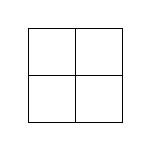
\begin{tikzpicture}[scale=0.6] \fill[white] (0,0) rectangle (2,2); \draw (0,0) grid (2,2); \end{tikzpicture}
\fillwithdottedlines{23mm}

\question[4] Shade the following sets : $A \cup B, \quad A \cap B \cap C, \quad \overline{B} \cap A, \quad (A \cap B) \cup \big(C \setminus (A \cup B) \big)$.

\fullwidth{

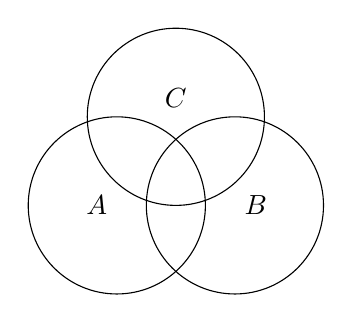
\begin{tikzpicture}[scale=0.75]
\fill[white] (-1,0) circle (1.5); 
\fill[white] (1,0) circle (1.5); 
\fill[white] (0,1.5) circle (1.5); 
	    
\draw(-1,0) circle (1.5) node[left, black] {$A$};
\draw (1,0) circle (1.5) node[right, black] {$B$};
\draw (0,1.5) circle (1.5) node[above, black] {$C$};
    
\end{tikzpicture}
\hfill
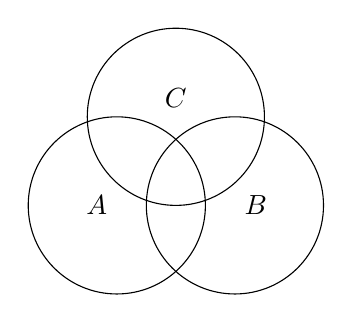
\begin{tikzpicture}[scale=0.75]
\fill[white] (-1,0) circle (1.5); 
\fill[white] (1,0) circle (1.5); 
\fill[white] (0,1.5) circle (1.5); 
	    
\draw(-1,0) circle (1.5) node[left, black] {$A$};
\draw (1,0) circle (1.5) node[right, black] {$B$};
\draw (0,1.5) circle (1.5) node[above, black] {$C$};
    
\end{tikzpicture}
\hfill
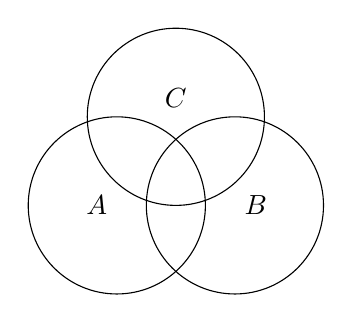
\begin{tikzpicture}[scale=0.75]
\fill[white] (-1,0) circle (1.5); 
\fill[white] (1,0) circle (1.5); 
\fill[white] (0,1.5) circle (1.5); 
	    
\draw(-1,0) circle (1.5) node[left, black] {$A$};
\draw (1,0) circle (1.5) node[right, black] {$B$};
\draw (0,1.5) circle (1.5) node[above, black] {$C$};
    
\end{tikzpicture}
\hfill
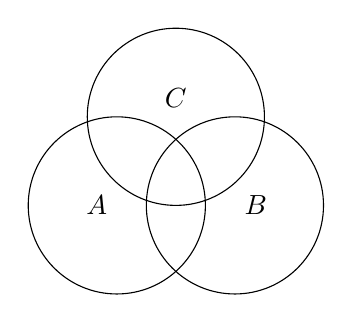
\begin{tikzpicture}[scale=0.75]
\fill[white] (-1,0) circle (1.5); 
\fill[white] (1,0) circle (1.5); 
\fill[white] (0,1.5) circle (1.5); 
	    
\draw(-1,0) circle (1.5) node[left, black] {$A$};
\draw (1,0) circle (1.5) node[right, black] {$B$};
\draw (0,1.5) circle (1.5) node[above, black] {$C$};
    
\end{tikzpicture}
\hfill
}


\question There are 160 third year students in a given high school, 70 of whom are in the bilingual program, 100 are enrolled in MA1, and 40 who are both in the bilingual program and enrolled in MA1. 
\begin{parts}
\part[3] Represent the situation as a Venn diagram. \emph{(Remember the universe as a box around your sets!)}

\vfill

\part[2] Pick a third year student at random. Compute the probability that
\begin{enumerate}
\vspace{4mm}
\item they are not in the bilingual program : \dotfill
\vspace{4mm}
\item they are enrolled in MA1 but are not in the bilingual program : \dotfill    
\end{enumerate}
\vspace{4mm}
\part[1] Pick a third year not in bilingual. What is the probability they are enrolled in MA1? \dotfill
\end{parts}


\question[0] \textbf{Bonus.} A taxi can carry at most 5 passengers and will make two journeys to transport 8 passengers from their hotel to the airport. Determine the number of different ways in which the people for the first journey may be selected. 

\emph{Work on the back, then answer here :} \dotfill

\end{questions}


\begin{tcolorbox}

\textbf{Name of marker:} 

\begin{center}
\gradetable[h][questions]
\end{center}

\end{tcolorbox}


\end{document}

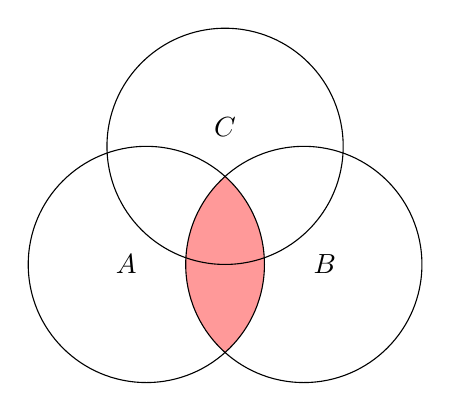
\begin{tikzpicture}
\fill[white] (-1,0) circle (1.5); 
\fill[white] (1,0) circle (1.5); 
\fill[white] (0,1.5) circle (1.5); 
	
    % Refill only A cap B
    \begin{scope}
        \clip (-1,0) circle (1.5);
        \fill[red!40] (1,0) circle (1.5);
    \end{scope}
    
    % Draw set A
    \draw(-1,0) circle (1.5) node[left, black] {$A$};

    % Draw set B
    \draw (1,0) circle (1.5) node[right, black] {$B$};

    % Draw set C without filling
    \draw (0,1.5) circle (1.5) node[above, black] {$C$};
    
\end{tikzpicture}
\hfill
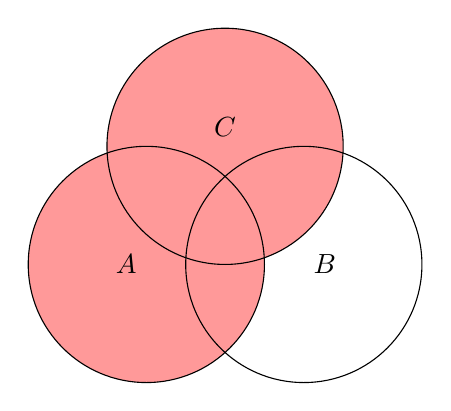
\begin{tikzpicture}
\fill[white] (-1,0) circle (1.5); 
\fill[white] (1,0) circle (1.5); 
\fill[white] (0,1.5) circle (1.5); 

    % Refill only A and C
   \fill[red!40] (0,1.5) circle (1.5);
   \fill[red!40] (-1,0) circle (1.5);
   
    % Draw set A
    \draw (-1,0) circle (1.5) node[left, black] {$A$};

    % Draw set B without filling
    \draw (1,0) circle (1.5) node[right, black] {$B$};

    % Draw set C
    \draw (0,1.5) circle (1.5) node[above, black] {$C$};
   
\end{tikzpicture}
\hfill
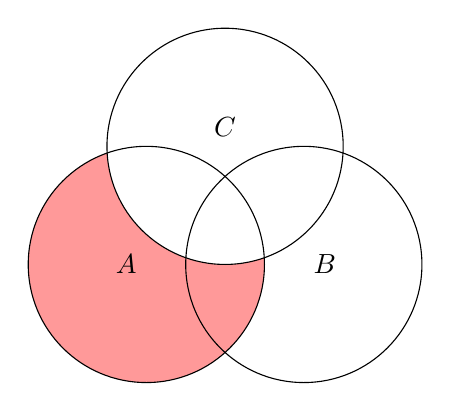
\begin{tikzpicture}
% Refill only A not C
\fill[white] (1,0) circle (1.5); 
\fill[red!40] (-1,0) circle (1.5); 
\fill[white] (0,1.5) circle (1.5); 
   
    % Draw set A
    \draw (-1,0) circle (1.5) node[left, black] {$A$};

    % Draw set B without filling
    \draw (1,0) circle (1.5) node[right, black] {$B$};

    % Draw set C
    \draw (0,1.5) circle (1.5) node[above, black] {$C$};
   
\end{tikzpicture}